\documentclass[11pt]{article}
\usepackage{hyperref, graphicx, enumerate, tikz, pdfpages, float}

\def\Name{Haojun Li}
\def\SID{24261499}
\def\Session{Fall 2015}

\title{Project Arctic}
\author{\Name, SID \SID}
\date{}

\renewcommand{\baselinestretch}{1.5}
\newcommand{\tab}{\hspace*{25pt}}

\newenvironment{abc}{\begin{enumerate}[{(}a{)}]}{\end{enumerate}}
\newenvironment{123}{\begin{enumerate}[1{.}]}{\end{enumerate}}

\graphicspath{ {images/} }

\textheight=9in
\textwidth=6.5in
\topmargin=-.75in
\oddsidemargin=0.25in
\evensidemargin=0.25in

\begin{document}
\maketitle
\begin{figure}[ht]
	
\includegraphics[scale=0.5]{icon.png}
	\centering
\end{figure}

\newpage
\section{Video}
The link to the video is \url{https://www.youtube.com/watch?v=F6yal5gOfdc}

\section{Description/Walkthrough}
\tab This application is designed for simplicity and minimum actions needed to get the 
user the information needed. Once the app is launched, it automatically asks the user how many
amount (reps/mins) of activity the user has done. While the user was inputing the amount, the
list instantly and automatically updates to reflect the user as he/she was typing. User
are able to change the activity from the spinner, and the unit (reps/mins) automatically
switches to the correct one. Then, user can switch to the next tab to input just the calorie
they want to burn and the application will tell the user the amount of different activities
neede to burn the calorie, along with the correct units.\\
\tab User are also able to change their weights in the settings tab on the menu button on
the top right coner. Once the settings are changed, the calories and list automatically updates
once the user are back to the main screen, minimizing user's need to click buttons and thus
simplify the process.

\section{Screenshots}
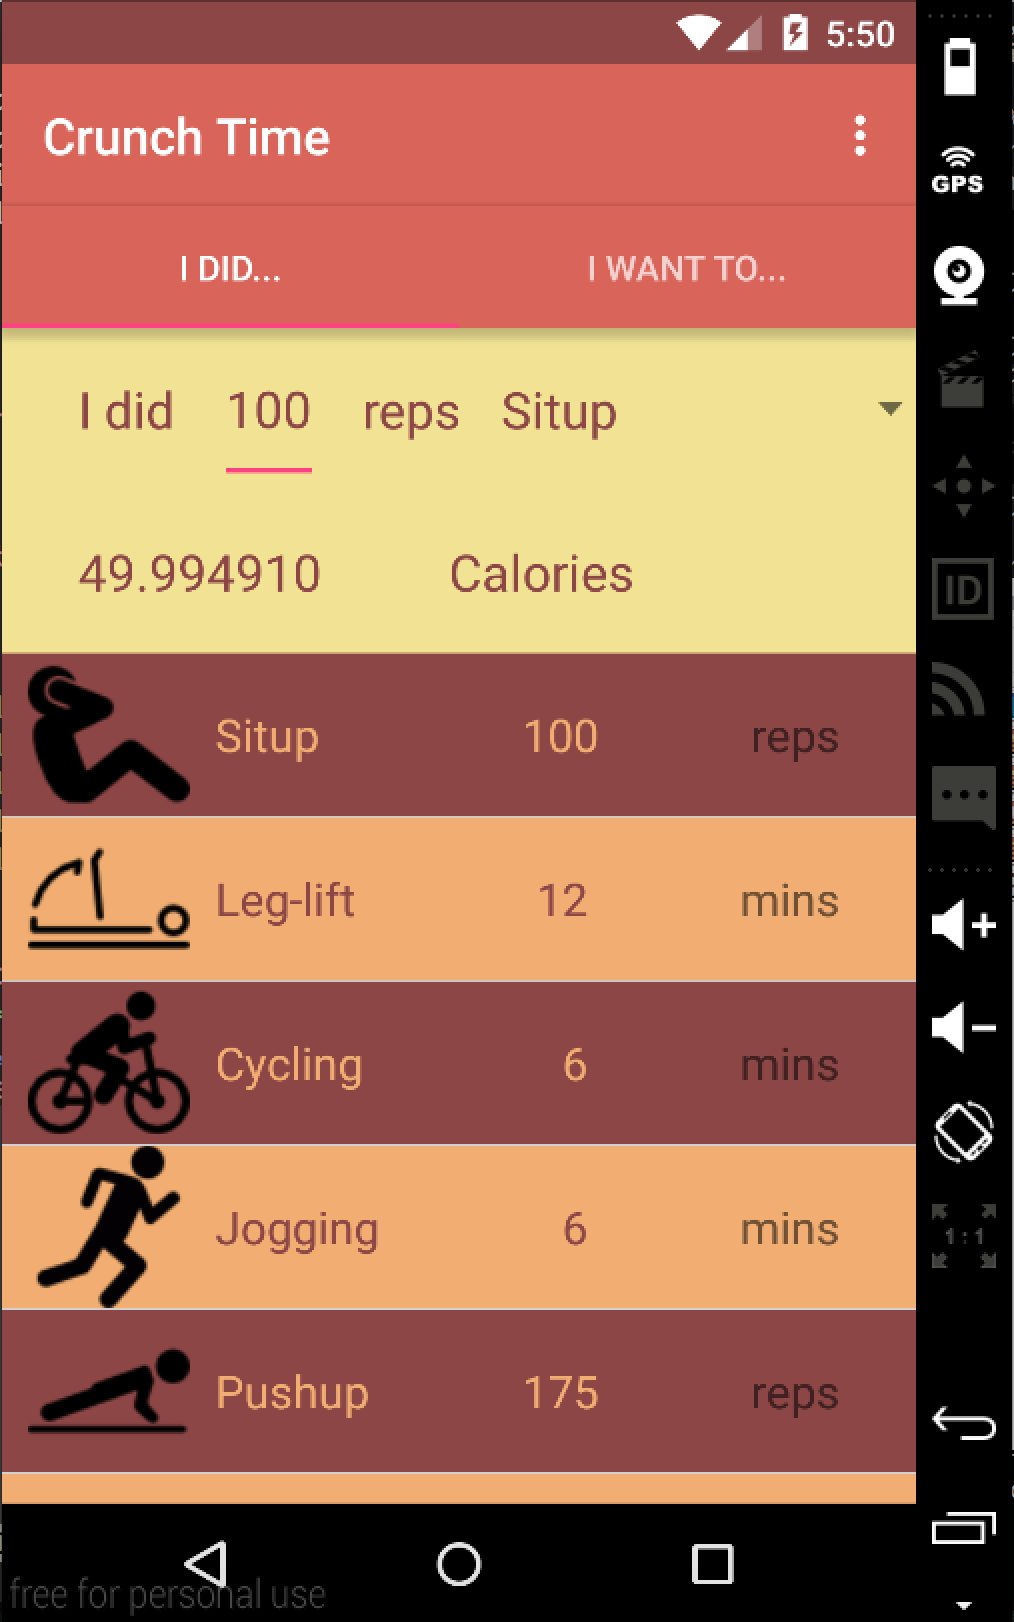
\includegraphics[scale=0.3]{shot1.png}\\
This screenshot is when the user inputed 100 in the input box.\\
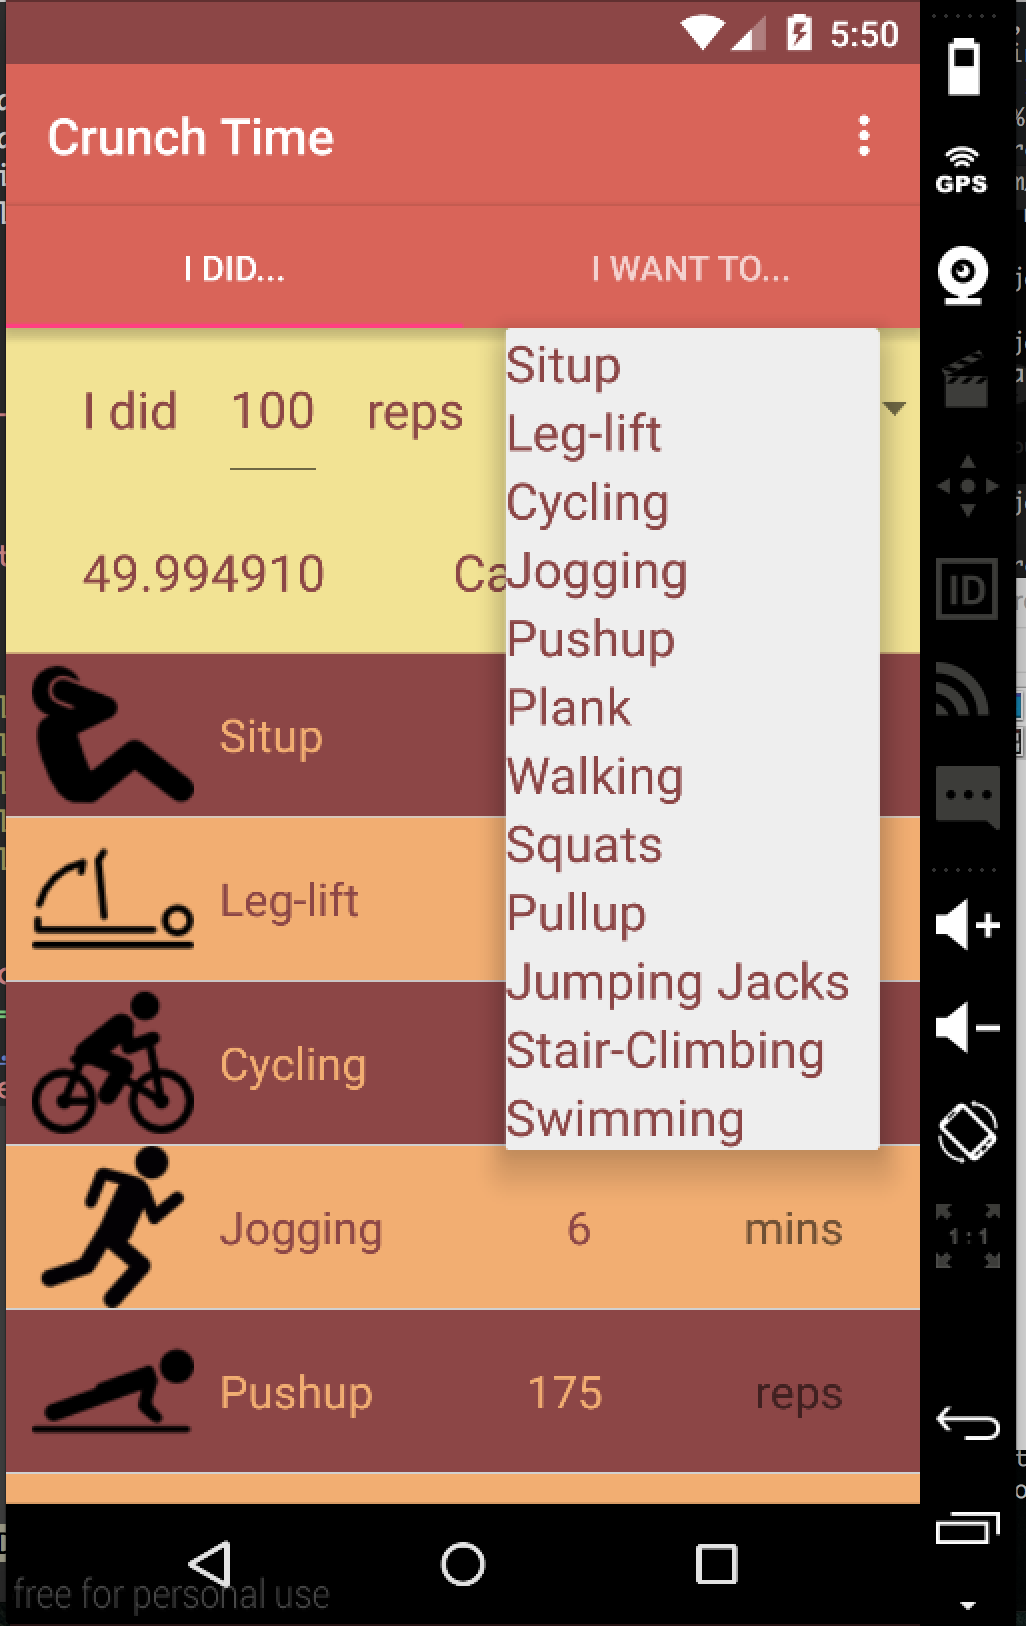
\includegraphics[scale=0.3]{shot2.png}\\
User are able to change the activity in this spinner.\\
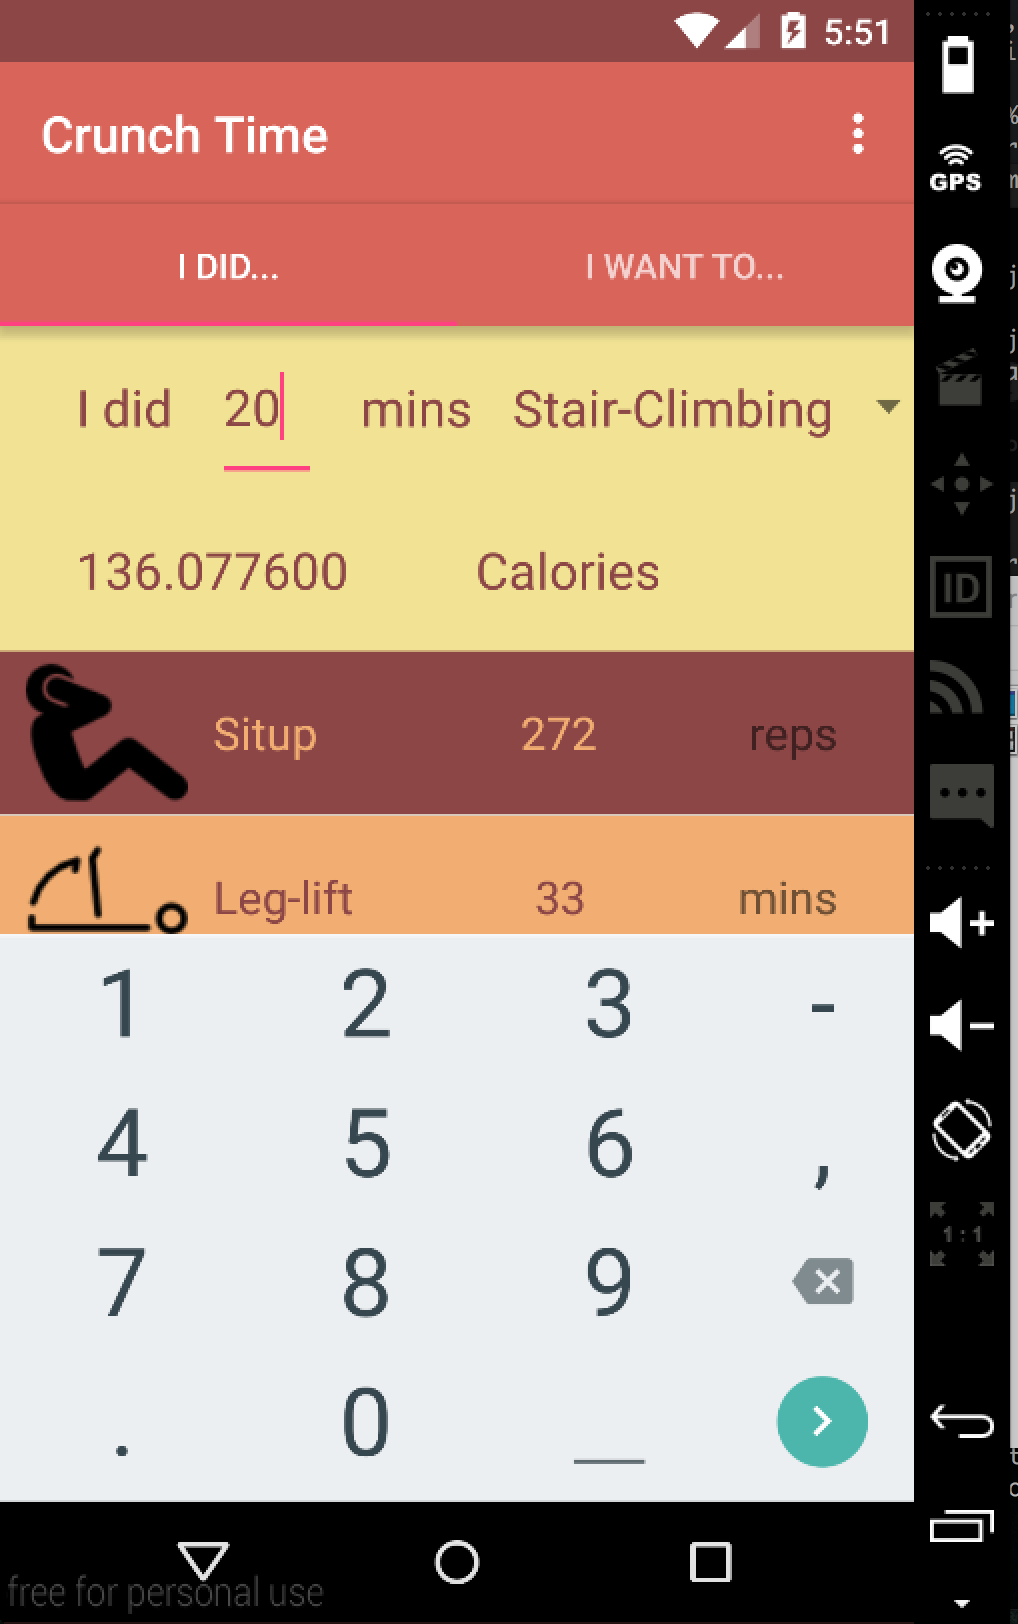
\includegraphics[scale=0.3]{shot3.png}\\
The unit automatically changes and the user are able to input from keyboard.\\
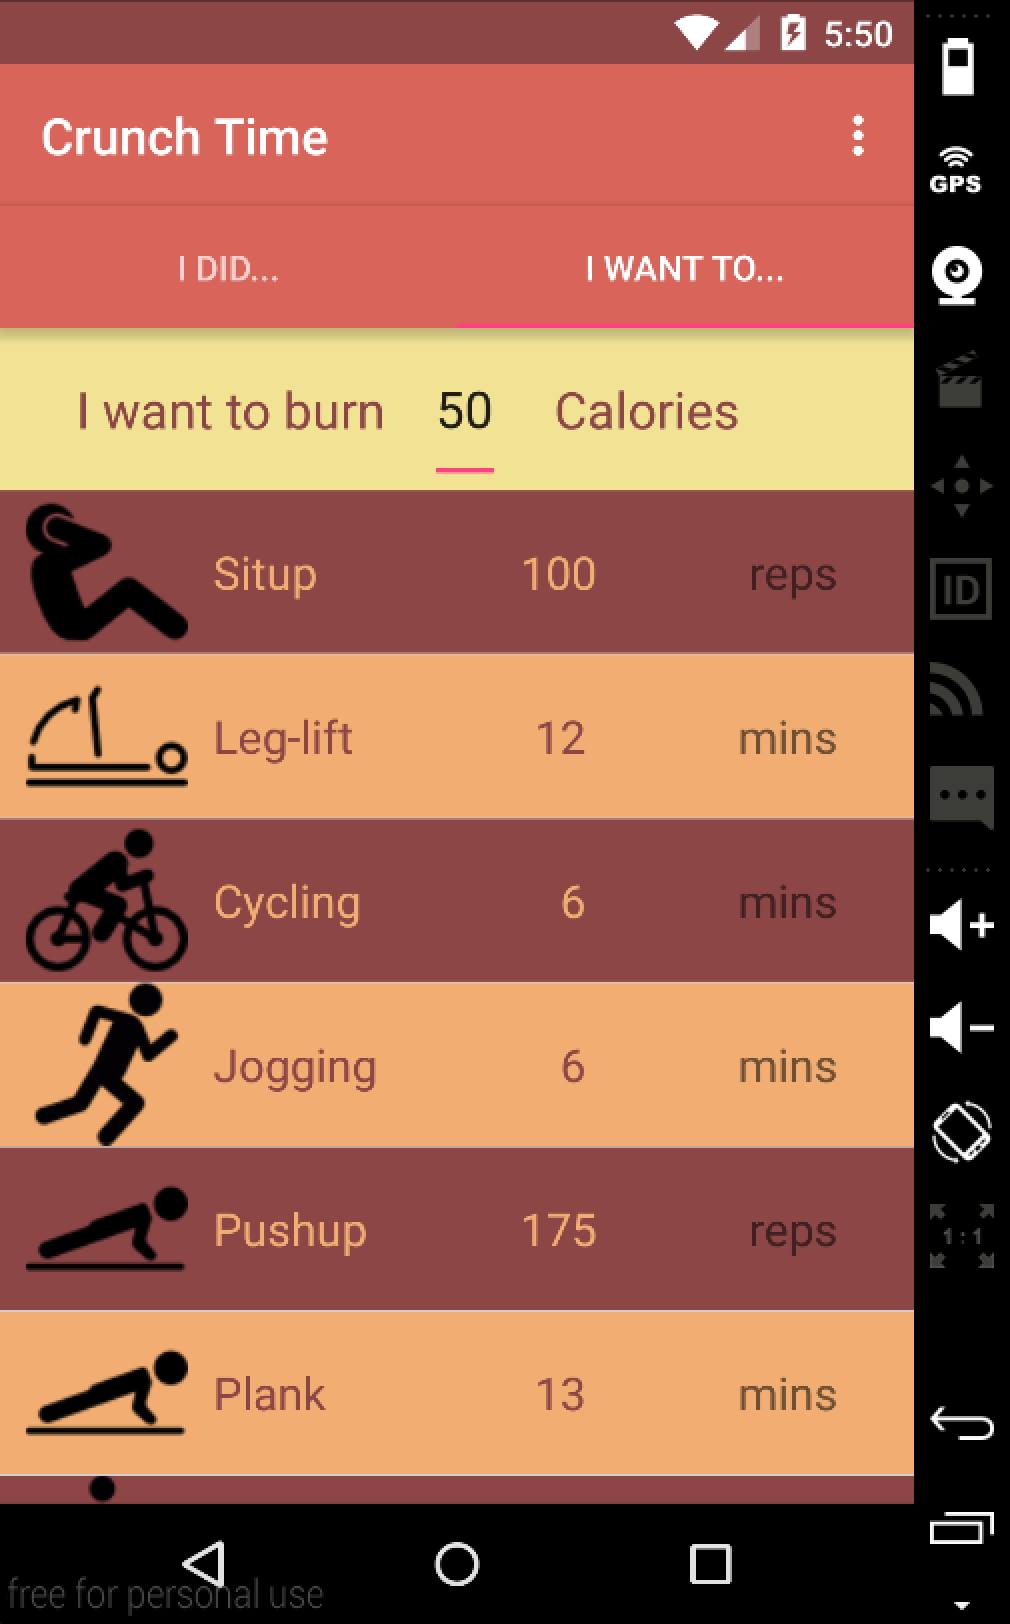
\includegraphics[scale=0.3]{shot4.png}\\
On the second tab, the user can input calories and get the amount needed for each activity.\\
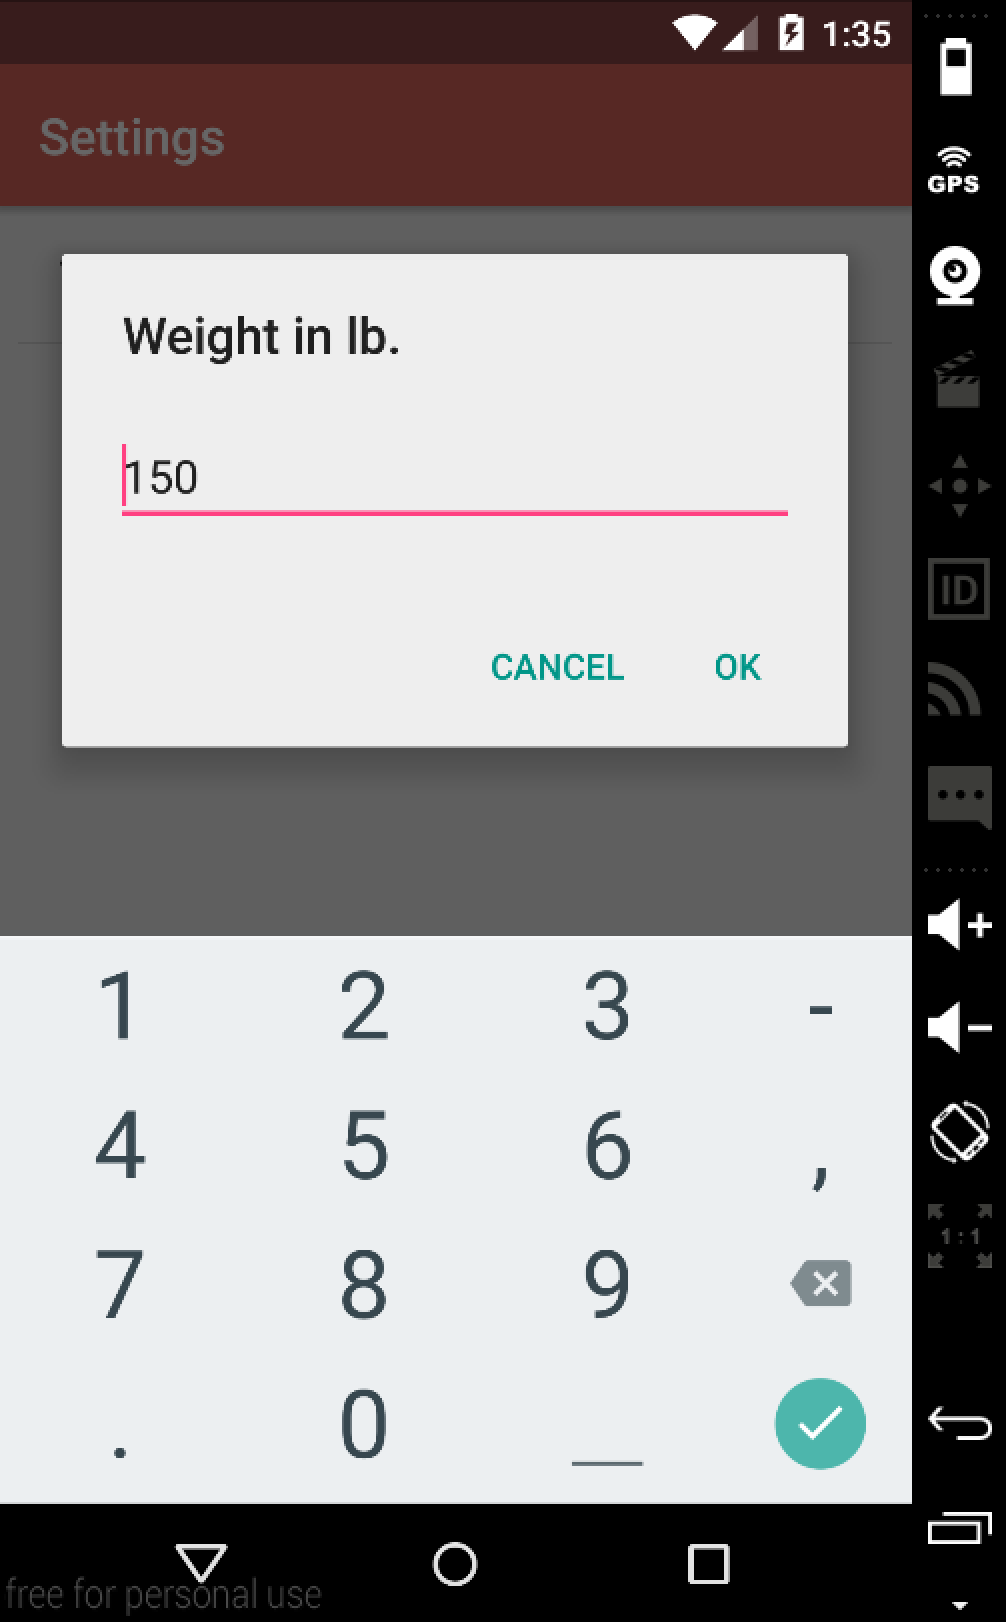
\includegraphics[scale=0.3]{shot5.png}\\
On the settings page, the user can change the weight to reflect more accurate calculation.\\

\section{GitHub}
The \href{https://github.com/cs160-sp16/prog-01-crunch-time-LithiumH}{GitHub Repo} is linked
here: \url{https://github.com/cs160-sp16/prog-01-crunch-time-LithiumH}


\end{document}
